\documentclass[11pt]{article}
\usepackage[a4paper,margin=1in]{geometry}
\usepackage[T1]{fontenc}
\usepackage{amsmath,amssymb}
\usepackage{booktabs,tabularx,tikz}
\usepackage{listings}
\usetikzlibrary{arrows.meta,positioning,shapes.geometric}
\usepackage[numbers,sort&compress]{natbib}
\usepackage[hidelinks]{hyperref}
\lstset{basicstyle=\ttfamily\scriptsize,breaklines=true,columns=fullflexible,
  keepspaces=true,showstringspaces=false,frame=single,xleftmargin=1em,
  xrightmargin=1em}
\newcommand{\E}{\mathcal E}
\newcommand{\pr}{\operatorname{pr}}
\title{Lie Symmetry Reduction near an Exceptional Transport Exponent:\\
An SVE-Informed Framework for Semi-Analytical Neural Approximation}
\author{}
\date{}
\begin{document}
\maketitle
\begin{abstract}
We formulate a bounded framework for reducing parameter-dependent nonlinear partial
differential equations through Lie symmetries and learning unresolved reduced
profiles. A shallow-water master equation provides a test of symmetry
persistence near an exceptional transport exponent. The methodology separates
classification, admissible reduction, analytical approximation, and neural
correction. Decoherence-in-quantum-fluid work motivates a later cross-scale
extension, but is not treated as a mechanism in the classical SVE benchmark.
We separate two literature baselines, a pure symbolic reduction, and a
certificate-gated fused prototype. The resulting experiments locate where the
neural correction helps and where conventional integration remains preferable;
a uniform neural error certificate remains open.
\end{abstract}

\section{Introduction}
Symmetry is a transformation that maps an object unchanged to a new space. It converts geometric information into analytical constraints on nonlinear
dynamics.

This paper investigates how Lie reduction can produce exact or
approximate solution families for parameter-dependent PDEs, with neural
approximation assigned to unresolved reduced profiles. The objective is a
tractable, interpretable method for mathematical physics and engineering,
with separate control of approximation and symmetry-breaking residuals.

The motivating example is the Saint--Venant--Exner (SVE) master equation of
Paliathanasis, Leon, and Leach \cite{ap}:
\begin{equation}
\E_m[\phi]=D_t\!\left(\phi_s\phi_{tt}-g\frac{\phi_{ss}}{\phi_s^2}\right)
-g\beta_{\rm tr} D_s\!\left(\phi_t^{m-1}\frac{\phi_{ts}}{\phi_s}\right)=0.
\label{eq:sve}
\end{equation}
Here $\phi(t,s)$ is particle position, $s$ a material label, and
$\beta_{\rm tr}=mA_g\xi$
the transport coefficient. Its reported point-symmetry algebra enlarges at
$m=3$. Parameter perturbation therefore challenges both classification and
reduction: an invariant ansatz at the exceptional value need not survive
nearby. We retain the published scalar equation as our benchmark; its physical
SVE interpretation requires resolving the bed-transport term identified by
the Eulerian-to-Lagrangian chain rule.

Quantum mechanics supplies a limited analogy: perturbations can destroy an
enhanced symmetry. For the isotropic oscillator,
$H_0=\hbar\omega(\sum_i a_i^\dagger a_i+k/2)$ and
$E_{ij}=a_i^\dagger a_j$ satisfy
\begin{equation}
[H_0,E_{ij}]=0,\qquad
[E_{ij},E_{\ell r}]=\delta_{j\ell}E_{ir}-\delta_{ir}E_{\ell j}.
\end{equation}
Their skew-Hermitian combinations generate $U(k)$; perturbations can reduce
this symmetry \cite{tong}. First-order continuation requires cancellation of
the corresponding symmetry defect. This is an analogy for testing, not
assuming, persistence near $m=3$. Noether's correspondence yields a conserved
current only for a variational symmetry \cite{noether}.

The decoherence literature gives distinct precedents. A Lindblad symmetry
analysis characterizes continuous symmetries and conserved quantities under
dissipation, where their unitary-system correspondence changes
\cite{lindbladsy}. A Caldeira--Leggett open-quantum-system study expands a
reduced density matrix near its diagonal,
truncates the resulting moment hierarchy, and obtains dissipative hydrodynamic
equations approaching compressible Navier--Stokes at late times
\cite{decohydro}. A separate Lindblad study examines perturbations and
discrete CP/CPT symmetry constraints, not Lie point symmetries of an engineering
PDE \cite{lindblad}. Neither derives classical water-wave or SVE equations.
For this project, decoherence is therefore a motivation for asking how
micro-to-macro closure can change a model; it is not a term in \eqref{eq:sve}.
Any water-specific extension must instead derive its scale bridge from the
chosen fluid, sediment, and bed-load closures.
A current classical example derives a shallow-water moment system from a
vertically resolved water-sediment Navier--Stokes model and couples it to
suspended-load and Exner bed-load balances with erosion and deposition
\cite{parvin}. This supplies a concrete engineering scale bridge without
invoking quantum decoherence.

\section{Preliminaries: from transformations to reduced equations}
Let $x=(x^1,\ldots,x^p)$ denote independent coordinates and
$u=(u^1,\ldots,u^q)$ field coordinates. A physical field is a section
$u=f(x;\lambda)$ of the local bundle $M\times\mathbb R^q\to M$, with fixed model
parameters $\lambda$. Reserve $p$ for independent variables, $q$ for fields,
$r$ for equations and $n$ for differential order. The jet $j^nf$ records
derivatives through order $n$; a PDE system is the submanifold
$\Delta_A(x,u^{(n)};\lambda)=0$, $A=1,\ldots,r$, wherever its defining
constraints have full rank.

A local Lie-group action transforms points and, when the transformed graph
remains a graph, fields:
\begin{align}
S_\varepsilon(x,u)&=(\bar x,\bar u),&
f_\varepsilon(\bar x;\lambda)&=\bar u\big|_{u=f(x;\lambda)},\\
\bar x^\mu&=x^\mu+\varepsilon\zeta^\mu+O(\varepsilon^2),&
\bar u^\alpha&=u^\alpha+\varepsilon\eta^\alpha+O(\varepsilon^2).
\end{align}
Thus $\varepsilon$ labels a group displacement, not a model perturbation.
The infinitesimal vector field and its characteristic are
\begin{equation}
X=\zeta^\mu\partial_{x^\mu}+\eta^\alpha\partial_{u^\alpha},
\qquad Q^\alpha=\eta^\alpha-\zeta^\mu u^\alpha_\mu.
\end{equation}
Repeated indices are summed. At fixed coordinates,
$\partial_\varepsilon f_\varepsilon^\alpha|_0=Q^\alpha[j^1f]$:
the characteristic subtracts apparent field change caused by coordinate
motion. Prolongation applies the chain rule to derivatives \cite{olver}:
\begin{align}
\pr^{(n)}X&=X+\sum_{\alpha,\,1\le|J|\le n}\eta_J^\alpha
\partial_{u_J^\alpha},\\
\eta_J^\alpha&=D_JQ^\alpha+\zeta^\mu u^\alpha_{J,\mu},
\qquad D_\mu=\partial_{x^\mu}+\sum_{\alpha,J}
u^\alpha_{J,\mu}\partial_{u_J^\alpha}.
\end{align}
Here $J$ is a derivative multi-index. Tangency to the equation manifold gives
\begin{equation}
\left.\pr^{(n)}X(\Delta_A)\right|_{\Delta=0}=0.
\label{eq:determining}
\end{equation}
Eliminate constrained derivatives, split in the remaining independent
derivatives, and solve the resulting determining equations for
$\zeta^\mu,\eta^\alpha$. Their solutions form a Lie algebra under commutators;
adjoint equivalence organizes inequivalent subgroup reductions.

For \eqref{eq:sve}, use $(x,u)=((t,s),\phi)$ and retain the source's
$X_i$ notation, with $S_i(\varepsilon)=\exp(\varepsilon X_i)$.
At $m=3$,
\begin{equation}
X_5=t\partial_t-2s\partial_s,
\quad S_5:(t,s,\phi)\mapsto(e^\varepsilon t,e^{-2\varepsilon}s,\phi),
\quad \phi=F(\sigma),\quad \sigma=st^2.
\end{equation}
Solving $X_5\sigma=0$ and $Q=0$ gives this invariant family; substitution
reduces the PDE to an ODE. Compatible data and regular group orbits are
required. Nonclassical symmetry instead imposes \eqref{eq:determining} on
the joint PDE and invariant-surface system $Q=0$, including differential
consequences; it is distinct from approximate symmetry.

Reserve $\delta=m-3$ for model perturbation: Kovalev's group parameter $a$
and perturbation parameter $\epsilon$ correspond to our $\varepsilon$ and
$\delta$, respectively \cite{kovalev}. Model parameters remain fixed under
$S_\varepsilon$; transformations changing them require an extended action.
For dimensionless $\phi_t>0$,
\begin{equation}
\phi_t^{2+\delta}=\phi_t^2\bigl(1+\delta\log\phi_t+O(\delta^2)\bigr).
\end{equation}
Expand both the equation and generator smoothly,
$\E_\delta=\E_0+\delta\E_1+O(\delta^2)$ and
$Y_\delta=Y_0+\delta Y_1+O(\delta^2)$, including the $m$-dependence of
$\beta_{\rm tr}$.
Here $Y_k$ denote perturbation coefficients; $X_i$ retain the source's basis labels.
If $\pr Y_0\E_0=c_0\E_0$, first-order persistence requires
\begin{equation}
\left.(\pr Y_1\E_0+\pr Y_0\E_1-c_0\E_1)\right|_{\E_0=0}=0.
\end{equation}
The correction must cancel the perturbation's symmetry defect; a solution
$Y_1$ is not guaranteed. For $z=(x,u)$ and generator coefficients
$V_0,V_1$, the approximate flow $\bar z=z_0+\delta z_1$ obeys
\begin{equation}
\frac{dz_0}{d\varepsilon}=V_0(z_0),\qquad
\frac{dz_1}{d\varepsilon}=DV_0(z_0)z_1+V_1(z_0),\qquad
z_0(0)=z,\quad z_1(0)=0.
\end{equation}
Kovalev's renormalization-group construction additionally extends the
equation manifold, finds its symmetries, and restricts them using the selected
boundary-value solution before reconstructing that solution; this restriction
must be derived for SVE.

\section{Related work and research position}
Symmetry-informed neural solution methods already exist. Akhound-Sadegh
et al.\ \cite{sympinn} penalize infinitesimal changes of the PDE residual;
this does not require every predicted solution to satisfy $Q=0$.
Jiao and Xiong \cite{jiao} exploit symmetry conditions for fundamental
solutions of linear PDEs. Kavousanakis et al.\ \cite{flow} learn time-varying
moving or rescaled coordinates and profiles through a PINN coupled to
index-2 differential-algebraic constraints; their examples include nonlinear
wave and spreading equations. LieSolver builds PDE solutions from known
symmetry transformations and fits initial/boundary data, but its reported
scope is linear homogeneous PDEs \cite{liesolver}. Thus combining Lie
reduction and PINNs is not a novelty claim. A one-dimensional SVE Lie analysis
also predates this study, and the selected Lagrangian source already reports
its symmetry algebra and similarity reductions \cite{sveold,ap}; discovery of
SVE symmetries or of $X_5$ is not claimed. The proposed contribution is
independent verification, persistence or obstruction under parameter
perturbation, and a parameter-conditioned neural correction to a reduced
analytical profile. The attached Navier--Stokes blow-up C/D manuscript is
used only as an example of a staged PDE construction and residual-correction
proof architecture; it does not establish an SVE, decoherence, or Lie-symmetry
method \cite{naviercd}. Otto et al.'s 2025 review unifies symmetry enforcement,
discovery, and promotion through Lie-derivative constraints; LieLAC uses
infinitesimal generators to canonicalize inputs for pre-trained models,
including neural PDE solvers \cite{otto,lieLAC}. These offer useful ML
interfaces, while the direct low-cost path here is exact symmetry reduction
before training. A 2025 master's thesis provides a recent worked account of
determining equations, gas-dynamic PDE systems, and symmetry-compatible
initial-boundary data \cite{beligiannis}. The 2024 algorithmic study of
approximate symmetry algebras highlights involutive completion and warns that
numerical rank/SVD methods can depend on base point and tolerance
\cite{approxalg}. An SDE preprint cited in the supplied draft learns generators while enforcing
Lie-bracket closure; this is adjacent evidence for learning algebra structure,
not a PDE classification result \cite{liestonet}. Effectiveness remains an
experimental question.

The supplied sources sharpen the scope of the classification claim. Liu and
Lou's 2024 review treats classical point reduction, conditional and CK-direct
methods, finite transformation groups, nonlocal methods, and supersymmetry as
distinct constructions; these should not be merged into one ``complete Lie
algebra'' \cite{liulou}. The supplied 2017 MSc dissertation works through
classical point reductions and nonclassical symmetries for drift-diffusion,
biased-diffusion, and KiSS population PDEs \cite{mathebula}. Hijazi's 2013 PhD
thesis compares classical, nonclassical, and potential-symmetry workflows on
coupled systems, including Burgers-type models, and discusses special cases
and time-dependent coefficients \cite{hijazi}. These are useful procedural
examples, but neither thesis is evidence for a new SVE result or a 2024--2026
ML method. For the low-cost study, first complete the classical local
point-algebra calculation; pursue conditional, potential/nonlocal, or other
symmetry notions only as separately named extensions motivated by the target
model and available conservation laws.

\section{Methodology: classify, reduce, and reconstruct}
\subsection{Formal PDE-system input}
The executable first version separates specification, candidate verification,
and reduction. It takes a supplied generator and local chart; it does not
require a claim of maximal symmetry classification before reducing a known
admitted subgroup. On a local bundle $E=\Omega\times\mathbb R^q\to\Omega$,
$\Omega\subset\mathbb R^p$, specify
\begin{equation}
\mathcal P_\lambda=
\bigl(\Omega,\Delta,\mathcal N,\mathcal A,
      \{(\gamma_b,\mathcal B_b)\}_{b=1}^{N_B};\lambda\bigr).
\label{eq:formal-problem}
\end{equation}
Here $\lambda$ consists of fixed real model parameters;
$\Delta_A(x,u^{(n)};\lambda)=0$, $A=1,\ldots,r$, are residual equations;
$\mathcal N$ lists nonzero expressions; and $\mathcal A$ records domain,
sign and smooth-branch predicates. No equality $r=q$ is required.
Data residuals $\mathcal B_b$ vanish on supplied base hypersurfaces
$\Gamma_b=\{x:\gamma_b(x;\lambda)=0\}$, restricted to the relevant local
domain. The order budget $n$ covers both equations and data. Thus
\begin{equation}
\Delta_A(j^nf;\lambda)=0,\qquad
N(j^nf;\lambda)\ne0\ (N\in\mathcal N),\qquad
\mathcal B_b(j^nf;\lambda)|_{\Gamma_b}=0.
\end{equation}
Predicates in $\mathcal A$ must also hold. A sampling distribution is a later
numerical choice, not part of the exact definition of a symmetry.

In Python, \texttt{PDEProblem} wraps the existing \texttt{DifferentialSystem}
and adds parameters, domain predicates and \texttt{DataCondition} records.
A jet $u^\alpha_J$, $J\in\mathbb N^p$, denotes a derivative coordinate, not a
sampled derivative value. Parameter symbols are disjoint from base and jet
coordinates; undeclared symbols and unevaluated derivative inputs are rejected.
The representation distinguishes polynomial, rational and nonpolynomial
dependence on jets. For the cubic master equation, multiplying by
$\phi_s^3$ produces a polynomial differential expression only on the retained
branch $\phi_s\ne0$. Generic real powers of $\phi_t$ require a specified smooth
real branch; the routine does not replace them by polynomial monomials.

\subsection{Verified reduction in a supplied chart}
The first algorithm supports one projectable point generator
$X=\zeta^i(x;\lambda)\partial_{x^i}
+\eta^\alpha(x,u;\lambda)\partial_{u^\alpha}$, with $p\ge2$.
Its input chart is
\begin{equation}
z=I(x)\in\mathbb R^{p-1},\qquad \rho=R(x),\qquad
x=H(z,\rho),\qquad u=C(x)U(z)+b(x).
\label{eq:reduction-chart}
\end{equation}
The profile coordinates $U$ and chart coordinates are fresh symbols.
The algorithm checks both inverse-coordinate identities, $XI^a=0$,
$XR\ne0$, and records the guards
$\det D_x(I,R)\ne0$ and $\det C\ne0$.
The orbit coordinate need not satisfy $XR=1$; for SVE we use $R=t$.
The affine field reconstruction includes field scaling and offsets, while
more general field transformations remain outside this implementation.

A supplied regular multiplier matrix $M(x;\lambda)$ is checked through the
off-shell identity
\begin{equation}
\pr^{(n)}X(\Delta)=M\Delta.
\label{eq:multiplier-identity}
\end{equation}
This is a sufficient, deliberately restricted test of the supplied generator.
Failure does not establish absence of all symmetries. Every denominator in
the supplied expressions is retained as a regularity condition. The routine
also verifies $Q^\alpha=0$ after the reconstruction substitution.

Derivative substitutions are generated recursively. If $P^\alpha_0=C U+b$,
then the pullback of a source jet is computed by
\begin{equation}
P^\alpha_{J+e_i}=\widehat D_i P^\alpha_J,\qquad
\widehat D_i=\partial_{x^i}
+\sum_{a=1}^{p-1}\sum_{\beta,K}
 (\partial_{x^i}I^a)U^\beta_{K+e_a}\partial_{U^\beta_K}.
\label{eq:pullback-recursion}
\end{equation}
Here $P$ has no explicit $z$ dependence before the inverse base substitution;
the coefficient functions use $x$ and profile-jet placeholders. The finite
jet budget is enforced. After setting $x=H(z,\rho)$, supplied nonzero factors
$a_A(x;\lambda)$ must give
\begin{equation}
\Delta_A[j^n(\mathcal TU)](H(z,\rho))
=a_A(H(z,\rho);\lambda)\,\mathcal R_A[j^nU](z).
\label{eq:chart-pullback}
\end{equation}
Any remaining $\rho$ dependence in $\mathcal R_A$ rejects this proposed
reduction. Zero equations are retained so the original equation count and
constraints remain traceable. The commuting square is
\[
\begin{array}{ccc}
U & \xrightarrow{\ \mathcal T\ } & f\\
{\scriptstyle\mathcal R}\downarrow &&
\downarrow{\scriptstyle\Delta}\\
\mathcal R[U] & \xrightarrow{\ \mathcal L_a\ } & \Delta[f],
\end{array}
\qquad (\mathcal L_a v)_A(x)=a_A(x)v_A(I(x)).
\]

\noindent\textbf{Local correctness statement.}
Assume the supplied maps are smooth on the recorded chart, its Jacobians
are nonzero, and all recorded branch and denominator conditions hold.
Then the verified identities imply
$\mathcal R[U]=0\Longleftrightarrow\Delta[\mathcal TU]=0$
for the reconstructed profiles on that chart. Invertibility of $C$ and the
base chart, together with $Q=0$, identifies these profiles locally with
invariant fields, after restricting to connected orbit segments.
Indeed, in chart coordinates $X$ acts along the nonvanishing orbit direction;
the reconstructed profile coordinates have zero derivative in that direction.
Equation~\eqref{eq:chart-pullback} and $a_A\ne0$ give both implications.
This classical local argument is not a new classification theorem
\cite{olver}. It establishes neither nonemptiness of the branch nor existence,
uniqueness or global continuation of solutions.

Data surfaces, data residuals and sign predicates are pulled back separately.
Conditions that retain $\rho$ are stored in the result and must still be
imposed; they are not discarded. The data status is
\texttt{pulled-back-only}, not a certificate of compatible initial-boundary
data. Differential completion and maximal classification retain their
separate, possibly incomplete statuses.

The executable entry points are \texttt{PDEProblem},
\texttt{ReductionChart} and \texttt{reduce\_in\_chart} in
\texttt{symm.generic}. The source-specific run is
\begin{lstlisting}[language=Python]
from symm.generic import reduce_in_chart
from symm.generic.sve_reduction import sve_scaling_case
problem, generator, chart, M = sve_scaling_case(m=3)
outcome = reduce_in_chart(
    problem, generator, chart, symmetry_multipliers=M)
print(outcome.certificate.status)
print(outcome.reduced_system.equations)
\end{lstlisting}
For this example, $\kappa=A_g\xi$ is fixed, $\beta_{\rm tr}=m\kappa$,
$I=st^2$, $R=t$, $H=(\rho,z/\rho^2)$, $C=1$, $b=0$,
$M=-1$ and $a_1=1/t$. At $m=3$ the routine reproduces
\eqref{eq:reduction}; at $m=4$ the same supplied multiplier identity fails.
This negative control concerns this generator and chart, not every possible
reduction at $m=4$.

\subsection{Model and admissibility}
First specify the scalar benchmark, parameter convention, physical domain,
and compatible data. For comparison with the full SVE system, rederive the
material-coordinate transformation: for an Eulerian quantity $b(t,x)$,
$\widetilde b(t,s)=b(t,\phi(t,s))$ gives
$\widetilde b_t=b_t+\phi_t b_x$. Any elimination of bed elevation must retain
this distinction and recover the original equations after reconstruction.
Until this audit is complete, results concern \eqref{eq:sve} itself.
Work locally where $\phi_s>0$, and, for noninteger exponents, on a specified
positive-velocity branch. Nondimensionalization precedes logarithmic expansion.

Compute the determining equations at generic $m$ and at $m=3$ separately;
division by $m-3$ would discard the exceptional branch. Verify each $X_i$
by prolongation, compute its commutators, and retain subgroups compatible
with the data. Solve their characteristic equations for invariants and check
the coordinate Jacobian. For a PDE with $p$ independent variables, an ODE
reduction requires $p-1$ independent orbit directions, subject to regularity
and transversality. A single symmetry does not generally reduce a higher
dimensional PDE to an ODE.

\subsection{What a complete classification means}
The completeness claim must name its transformation class. The primary target
is the maximal local \emph{point-symmetry Lie algebra} on each regular parameter
stratum: smooth transformations of $(x,u)$ whose prolonged fields are tangent
to the PDE jet manifold. This determines the identity component locally. It
does not include, without separate work, generalized or contact symmetries,
nonlocal or conditional symmetries, variational symmetries, or discrete maps.
For linear PDEs the point algebra may also contain an infinite-dimensional
solution-superposition ideal, so a finite polynomial ansatz cannot establish
maximality. A point symmetry of the differential equation is not automatically
a symmetry of its initial-boundary value problem: the data and domain must be
invariant too \cite{beligiannis}.

In practical terms, ``all'' means all solutions of the determining system in
the declared smoothness class, on the stated regular jet chart, for the
specified fixed-parameter stratum and point-transformation class. There is no
universal finite-degree ansatz that proves this for an arbitrary nonlinear
PDE. A completeness certificate therefore records: (a) the regular and
singular branches of the equation manifold; (b) all coefficient and rank
branches, including exceptional parameter values; (c) the complete solution
of, or involutive completion of, the determining PDEs for unrestricted
infinitesimals; and (d) substitution of the resulting basis into every
prolonged equation. The polynomial calculation below is a cheap candidate
search and an $m=3$ anchor, not that certificate. Symmetries of a specified
initial-boundary value problem are then the subgroup preserving its domain
and data.

For a parameterized model, first compute the equivalence group (which may
transform parameters), then classify admitted algebras for fixed parameter
values modulo that equivalence. Split exceptional strata before dividing by
parameter factors. The Lie algebra describes only the identity component;
for a global group, record the component sequence
$1\to G^0\to G\to\pi_0(G)\to1$ and determine $\pi_0(G)$ separately.
Reflections, reversals, permutations, and other disconnected components are
tested directly on the equation and domain. Topology and global coverage of a
Lie group are not recovered from infinitesimal determining equations alone.
Likewise, do not adjoin discrete maps to a Lie algebra. A semidirect product
is appropriate only after an actual action on the continuous group is defined
and the combined transformations are checked to preserve the PDE.

Keep three perturbation questions distinct: (i) exact symmetries at fixed
parameters; (ii) approximate continuation of a generator under
$\lambda=\lambda_0+\delta\lambda$; and (iii) equivalence transformations that
move the parameter. The first-order defect equation in the preliminaries
addresses (ii); its bracket closure is checked modulo $O(\delta^2)$. If the
equation itself changes in time, recompute the determining system for that
coefficient function. Numerical near-symmetry discovered by SVD is useful for
diagnosis, but is not an exact classification certificate \cite{approxalg}.

\subsection{Reproducible SymPy workflow on the SVE branch}
The following compact jet-space implementation uses SymPy's exact
differentiation, polynomial collection, and matrix nullspace operations. It
spells out the prolongation instead of relying on a black-box Lie solver;
the documented SymPy PDE interface includes utilities such as separation,
which are different from a general PDE symmetry classifier \cite{sympydocs}.
The code below computes candidates in a declared polynomial ansatz for the
regular $m=3$ branch. It does not compute the generic-$m$ algebra: that branch
needs a separate determining-system run and a branch-aware split of the
noninteger powers on $phi_t>0$. Increase the ansatz only after examining the
determining system; completeness requires solving that full linear
differential system, including its arbitrary-function branches, not merely
enlarging a finite polynomial trial space.

\begin{lstlisting}[language=Python]
import sympy as sp

t, s, m = sp.symbols("t s m", real=True)
g, Ag, xi_sed = sp.symbols("g Ag xi_sed", positive=True)
R = 3                         # order of the SVE master PDE
jets = {(i, j): sp.Symbol(f"u{i}{j}", real=True)
        for i in range(R + 2) for j in range(R + 2 - i)}
u = jets[(0, 0)]

def D(expr, axis):            # axis 0=t, 1=s; total derivative
    out = sp.diff(expr, (t, s)[axis])
    for (i, j), uj in jets.items():
        if i + j <= R:
            nxt = (i + (axis == 0), j + (axis == 1))
            out += sp.diff(expr, uj) * jets[nxt]
    return sp.expand(out)

Dt, Ds = lambda f: D(f, 0), lambda f: D(f, 1)
us, ut = jets[(0, 1)], jets[(1, 0)]
utt, uss, uts = jets[(2, 0)], jets[(0, 2)], jets[(1, 1)]
beta = m * Ag * xi_sed
E = Dt(us*utt - g*uss/us**2) - g*beta*Ds(ut**(m-1)*uts/us)
E3 = sp.cancel(E.subs(m, 3))

def prolong(tau, xi, eta, r=R):
    e = {(0, 0): eta}
    for n in range(1, r + 1):
        for i in range(n + 1):
            j = n - i
            if i: parent, axis = (i - 1, j), 0
            else: parent, axis = (i, j - 1), 1
            a, b = parent
            e[(i, j)] = sp.expand(
                D(e[parent], axis)
                - jets[(a + 1, b)] * D(tau, axis)
                - jets[(a, b + 1)] * D(xi, axis))
    return e

def prX(F, tau, xi, eta, r=R):
    e = prolong(tau, xi, eta, r)
    ans = tau*sp.diff(F, t) + xi*sp.diff(F, s) + eta*sp.diff(F, u)
    for (i, j), ej in e.items():
        if i + j and (i + j) <= r:
            ans += ej * sp.diff(F, jets[(i, j)])
    return sp.expand(ans)

# Candidate search only: total-degree <= 2 in (t,s,u).
mon = [t**a*s**b*u**c for a in range(3) for b in range(3-a)
       for c in range(3-a-b)]
def ansatz(prefix):
    cs = sp.symbols(f"{prefix}0:{len(mon)}")
    return sum(c*p for c, p in zip(cs, mon)), cs

tau, c_tau = ansatz("ct")
xi, c_xi = ansatz("cs")
eta, c_eta = ansatz("cu")
cvars = c_tau + c_xi + c_eta
lead = jets[(3, 0)]       # regular branch: solve E3 for phi_ttt
lead_rule = sp.solve(E3, lead, dict=True)[0]
determining = sp.cancel(prX(E3, tau, xi, eta).subs(lead_rule))
num = sp.together(determining).as_numer_denom()[0]
free_jets = [jets[J] for J in jets
             if 0 < sum(J) <= R and J != (3, 0)]
P = sp.Poly(num, *(free_jets + [t, s, u]), domain="EX")
eqs = P.coeffs()                       # split all free-jet monomials
M, rhs = sp.linear_eq_to_matrix(eqs, cvars)
basis = M.nullspace()                  # exact candidate generators
generators = []
for v in basis:
    gen = tuple(sp.expand(f.subs(dict(zip(cvars, v))))
                for f in (tau, xi, eta))
    test = sp.cancel(prX(E3, *gen).subs(lead_rule))
    assert sp.simplify(test) == 0       # verify each candidate on E3=0
    generators.append(gen)
check_x5 = sp.cancel(prX(E3, t, -2*s, 0).subs(lead_rule))
assert sp.simplify(check_x5) == 0       # independent m=3 anchor check
\end{lstlisting}

Read the steps as an executable protocol. First form the PDE using independent
jet symbols, not unevaluated derivatives of an unknown function. The total
derivative operator raises each jet index and the recursion constructs
$\eta_J=D_i\eta_{J-e_i}-u_{J-e_i,t}D_i\tau-u_{J-e_i,s}D_i\xi$.
Second, solve the regular PDE branch for a chosen leading jet and substitute
it into $\operatorname{pr}^{(3)}X(E)$. For the SVE equation the leading
coefficient is nonzero on $\phi_s>0$; record that condition and analyze
singular branches separately. Third, clear only denominators known nonzero on
the branch, split with respect to all remaining jets (and then the base
coordinates), and solve the resulting homogeneous linear system. The matrix
nullspace returns a basis within the stated ansatz. For a system, repeat the
criterion for every $E_A$ and eliminate a compatible set of leading jets;
check differential consequences whenever the system is not in a regular
solved form.

For generic symbolic $m$, the factors $\phi_t^{m+k}$ are not ordinary
polynomial monomials. Split them as distinct smooth functions on the chosen
$\phi_t>0$ branch, or analyze rational/integer $m$ strata separately; then
solve $m=3$ again without first dividing by $m-3$. For
$m=3+\delta$, expand powers as
$\phi_t^{2+\delta}=\phi_t^2(1+\delta\log\phi_t)+O(\delta^2)$ and retain the
logarithmic basis element in the split. To certify maximality, replace the
finite polynomial ansatz by unknown functions $\tau(t,s,\phi)$,
$\xi(t,s,\phi)$, and $\eta(t,s,\phi)$, integrate the determining PDEs (or
complete them to an involutive differential system), branch on every
parameter/rank condition, and verify the final basis by substitution. Exact
differential completion is the completeness gate; a numerical SVD or finite
degree ansatz is a discovery aid \cite{approxalg}.

For every basis element, run an independent invariance check by substituting
the solved-jet rules into $\operatorname{pr}^{(3)}X(E)$ and simplifying to
zero. Compute $[X_i,X_j]$ componentwise as
$X_i(\zeta_j,\xi_j,\eta_j)-X_j(\zeta_i,\xi_i,\eta_i)$; express each bracket
in the basis to obtain structure constants and check Jacobi. The adjoint
representation then supports the optimal-system calculation. For $X_5$,
verify $X_5(st^2)=0$ and $X_5(\phi)=0$, substitute $\phi=F(st^2)$ directly,
and simplify $t\E_3-\mathcal R_0[F]$ to zero. Finally exponentiate candidate
generators and check the finite transformation on the physical domain; local
infinitesimal validity alone does not establish a globally admissible action.

\subsection{Representation theory and low-cost ML interfaces}
Representations are useful after the infinitesimal algebra has been found;
they are not required to discover low-dimensional point symmetries. Compute
the commutator table and adjoint matrices first. The adjoint representation is
needed for classifying one-dimensional subalgebras. Compute the center,
derived algebra, solvable radical, and (when useful) Levi factor from the
commutator table; do not assume a direct or semidirect sum before verifying
closure and the action. Representations on the fields, jets, or learned
feature channels are useful when imposing equivariance. For a linear layer
$W$ with input and output infinitesimal representations $d\rho_{\rm in},
d\rho_{\rm out}$, the intertwining constraints are
$W d\rho_{\rm in}(X_i)=d\rho_{\rm out}(X_i)W$. Add these only if a
nontrivial equivariant architecture is warranted.

The least expensive ML path is: (1) exact symbolic reduction to invariant
coordinates; (2) represent the analytical profile plus a small correction
network in those coordinates; (3) reconstruct with the known group action;
(4) penalize the first-order defect only for the broken directions. This
reduces input dimension and avoids sampling the continuous group. If repeated
parameter/forcing queries are needed, learn an operator on reduced profiles.
If symmetry is unknown from data, estimate a candidate generator nullspace
from a discretized Lie-derivative operator, then pass candidates to the exact
symbolic verifier. A global canonical section may fail at singular orbits or
for topological reasons, so use local moving-frame charts and test their
overlap instead of assuming one canonicalization works everywhere
\cite{lieLAC}. The JMLR review frames enforcement, discovery, and
symmetry-promoting regularization as linear-algebraic problems, and LieLAC
offers a canonicalization socket when full group formulas are inconvenient
\cite{otto,lieLAC}. For a baseline PINN, a post-training correction
$F_{\rm PINN}+\omega_N C_\theta$ can target the residual left in the reduced
manifold; compare it against an equally budgeted direct correction. For an
LLM, the reliable role is orchestration: emit a typed PDE/generator/parameter
specification, call SymPy for prolongation, splitting, and verification, then
report the exact residual and unresolved branches. The language model itself
is not the completeness certificate.

\subsection{An explicit reduction anchor}
For $X_5$ at $m=3$, take $t>0$ and $\sigma=st^2$. Writing primes for
$d/d\sigma$, direct differentiation gives
\begin{equation}
\phi_s=t^2F',\qquad \phi_t=\frac{2\sigma F'}{t},\qquad
\phi_{tt}=\frac{2\sigma F'+4\sigma^2F''}{t^2}.
\end{equation}
Define the following expressions, rather than new model parameters:
\begin{align}
A[F]&=2\sigma(F')^2+4\sigma^2F'F''-g\frac{F''}{(F')^2},\\
B[F]&=8\sigma^2F'(F'+\sigma F'').
\end{align}
Since $D_t A=2\sigma A'/t$ and the transport term inside $D_s$ is
$t^{-3}B$, the reduced equation is
\begin{equation}
\E_3[F(st^2)]=t^{-1}\mathcal R_0[F],\qquad
\mathcal R_0[F]=2\sigma A'[F]-g\beta_{\rm tr} B'[F]=0,
\quad \beta_{\rm tr}=3A_g\xi.
\label{eq:reduction}
\end{equation}
This identity supplies a symbolic and numerical consistency check before
approximating $F$. It describes an invariant solution family, not arbitrary
initial data. Singular points of the reduced equation require separate analysis.

\subsection{Continuation near the exceptional exponent}
Solve the first-order symmetry condition for $Y_0=X_5$ before extending this
ansatz to $\delta\ne0$. If a deformation exists, construct its invariants
to the same order and substitute them into the perturbed equation. If it
does not, use a surviving subgroup or retain the additional independent
variable. In particular, the unrestricted correction
$\phi=F(st^2)+\delta\psi(t,s)+O(\delta^2)$ satisfies
\begin{equation}
D_\phi\E_0[F]\,\psi+\E_1[F]=0,
\end{equation}
with $D_\phi\E_0$ the linearization in the field. This is generally a PDE;
writing $\psi=F_1(\sigma)$ without checking closure would impose an
unsupported reduction. Truncation accuracy is local and must be checked
uniformly on the chosen domain.

\subsection{Time-dependent coefficient perturbations}
Keep two perturbations separate. The primary continuation is the constant
exponent $m=3+\delta$, including the induced change in
$\beta_{\rm tr}=mA_g\xi$.
A later nonautonomous test may prescribe
$\beta_{\rm tr}(t)=\beta_{\rm tr,0}[1+\delta q(t)]$ with fixed $m=3$; this is a controlled
coefficient perturbation, not a newly derived SVE closure. Time-dependent
boundary or initial data are a separate compatibility test. For each case,
recompute the determining equations and first-order symmetry defect rather
than assuming $X_5$ persists. A time-varying exponent $m(t)$ is excluded unless
a constitutive derivation justifies it. A frozen-time or adiabatic approximation
is admissible only after a slow-variation scale is stated and checked.

\begin{figure}[htbp]
\centering
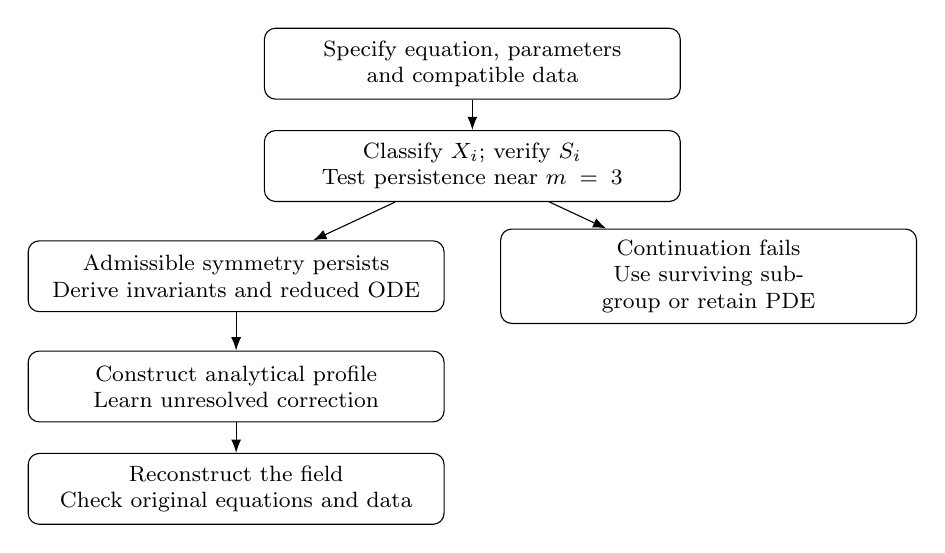
\begin{tikzpicture}[>=Latex,
 box/.style={draw,rounded corners,align=center,font=\footnotesize,
 text width=5cm,minimum height=9mm,inner sep=4pt}]
\node[box] (model) at (0,0) {Specify equation, parameters\\and compatible data};
\node[box] (class) at (0,-1.3) {Classify $X_i$; verify $S_i$\\Test persistence near $m=3$};
\node[box] (yes) at (-3,-2.7)
 {Admissible symmetry persists\\Derive invariants and reduced ODE};
\node[box] (no) at (3,-2.7)
 {Continuation fails\\Use surviving subgroup or retain PDE};
\node[box] (learn) at (-3,-4.1)
 {Construct analytical profile\\Learn unresolved correction};
\node[box] (check) at (-3,-5.4)
 {Reconstruct the field\\Check original equations and data};
\draw[->] (model)--(class);
\draw[->] (class)--(yes); \draw[->] (class)--(no);
\draw[->] (yes)--(learn);
\draw[->] (learn)--(check);
\end{tikzpicture}
\caption{Decision flow. Follow the neural ODE branch only after a valid
reduction is established; failed continuation returns to mathematical analysis.}
\end{figure}

\section{Machine-learning construction and comparison design}
\subsection{Learn the part left unresolved by analysis}
For an admissible reduced problem, let $F_{\mathrm{an}}$ denote a provisional
analytical approximation and $\lambda$ its physical parameters and admissible
integration constants. Construct
\begin{equation}
\widehat F_\theta(\sigma;\lambda)=F_{\mathrm{an}}(\sigma;\lambda)
+\omega_N(\sigma;\lambda)N_\theta(\sigma;\lambda),\qquad
\widehat\phi_\theta=\mathcal T_\lambda[\widehat F_\theta],
\label{eq:neural}
\end{equation}
where $\mathcal T_\lambda$ is the derived reconstruction map. The factor
$\omega_N$
preserves known linear constraints. For prescribed Taylor coefficients
through order $K$ at a regular point $\sigma_0$, one possible choice is
$F_{\mathrm{an}}=P_K$ and $\omega_N=(\sigma-\sigma_0)^{K+1}$.
This example does not select Taylor expansion as the final method.
Analytically constrained neural trial functions have a longstanding precedent
\cite{lagaris}; the research question is how to construct their analytical
part from the perturbed symmetry structure.

Train on collocation coordinates and parameter values, not necessarily
solution labels. For a derived residual $\mathcal R_\lambda$ and any constraints
$\mathcal B_\lambda$ not imposed exactly, use
\begin{equation}
\mathcal L(\theta)=
\left\langle\|\mathcal R_\lambda[\widehat F_\theta]\|^2\right\rangle_{\mathcal C}
+w_B\left\langle\|\mathcal B_\lambda[\widehat F_\theta]\|^2\right\rangle
+w_D\left\langle\|\mathcal H\widehat\phi_\theta-y\|^2\right\rangle_{\mathcal D}.
\end{equation}
Brackets denote sample averages; $\mathcal H$ is an observation operator.
Omit the final term when no measurements are supplied. Scale residual
components using the nondimensional equations, and document how weights
are chosen. Use symbolic differentiation for reduction identities and
automatic differentiation for neural residuals. Choose network capacity,
sampling density, and stopping criteria by validation rather than fixed
unmotivated numerical values.

\begin{figure}[htbp]
\centering
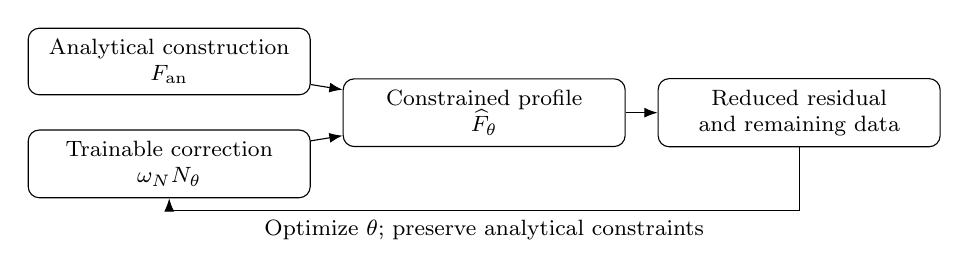
\begin{tikzpicture}[>=Latex,
 box/.style={draw,rounded corners,align=center,font=\footnotesize,
 text width=3.3cm,minimum height=8mm,inner sep=4pt}]
\node[box] (a) at (-4,0) {Analytical construction\\$F_{\mathrm{an}}$};
\node[box] (n) at (-4,-1.3) {Trainable correction\\$\omega_N N_\theta$};
\node[box] (f) at (0,-.65) {Constrained profile\\$\widehat F_\theta$};
\node[box] (r) at (4,-.65) {Reduced residual\\and remaining data};
\draw[->] (a)--(f); \draw[->] (n)--(f); \draw[->] (f)--(r);
\draw[->] (r.south)--++(0,-.8)-| node[pos=.25,below,font=\footnotesize]
 {Optimize $\theta$; preserve analytical constraints} (n.south);
\end{tikzpicture}
\caption{Neural construction. The analytical component and reconstruction
are specified by the reduction; optimization adjusts the unresolved profile.}
\end{figure}

\subsection{Comparisons that isolate each contribution}
The following comparison design isolates each contribution. All methods must
target the same admissible solution and data.
\begin{center}
\small
\begin{tabularx}{\linewidth}{@{}lX@{}}
\toprule
Construction & Question isolated \\
\midrule
Analytical approximation alone & How much does neural correction add? \\
Reduced PINN without analytical part & Does the analytical construction help training? \\
Direct PDE PINN & What benefit comes from reducing coordinates? \\
PDE PINN with symmetry loss \cite{sympinn} & Does explicit reduction help beyond regularization? \\
Converged conventional reduced solver & Is the learned profile accurate and cost-effective? \\
\bottomrule
\end{tabularx}
\end{center}
Use exact profiles when available, otherwise independently converged
reference solutions. Report profile error, reconstructed PDE residual,
data mismatch, runtime, and variation across training seeds. Separate
interpolation from held-out parameter tests. Symmetry-generated copies
of one profile stay in the same data split. Test both the exceptional case
and nearby admissible parameters; failure of symmetry continuation is itself
a mathematical result, not a training failure.

Evaluate the original PDE on independent points even when training uses
only a truncated ODE. A small reduced residual alone does not bound solution
error: such a bound additionally requires stability of the reduced problem,
controlled reconstruction, and a perturbation-remainder estimate.
Compare error versus computational budget rather than assume that fewer
coordinates guarantee faster training.

\section{Implemented three-layer baseline and fused prototype}
\subsection{Reported ML baselines kept outside the Lie pipeline}
The ML-only executable imports no Lie-reduction code.  Its first experiment is
a bounded fixed-IVP reproduction of the Duffing comparison in the Taylor-model
PINN paper \cite{tmpinn},
\[
 \dot x=y,\qquad \dot y=x-x^3-\delta_Dy,
 \quad (x(0),y(0),\delta_D)=(-0.224,-0.269,0.327).
\]
Here $\delta_D$ is the Duffing damping coefficient and is unrelated to
$\delta=m-3$. All three methods use one hidden layer of width 64 and three
seeds. Table~\ref{tab:duffing} gives relative $L^2$ medians after 3000 Adam
steps; the bracket is the full seed range for TM-PINN.
\begin{table}[htbp]
\centering\small
\begin{tabular}{@{}ccccc@{}}
\toprule
Horizon & vanilla PINN & higher-order PINN & TM-PINN & TM range \\
\midrule
$T=1$ & $2.050\times10^{-4}$ & $1.914\times10^{-4}$ & $7.585\times10^{-5}$
 & $[4.491\times10^{-5},1.001\times10^{-4}]$ \\
$T=3$ & $6.555\times10^{-2}$ & $9.841\times10^{-2}$ & $1.756$
 & $[8.678\times10^{-2},8.894]$ \\
\bottomrule
\end{tabular}
\caption{Bounded Duffing fixed-IVP reproduction. It tests the reported
short-time advantage and long-time degradation, not the paper's full
parameter-family solution map.}
\label{tab:duffing}
\end{table}

The second experiment follows the 2026 PINN--PIKAN logistic benchmark
\cite{pikan} with 100 uniform points, Adam step size $0.01$, 10000 iterations
and ten seeds. The MLP has 121 parameters; the PIKAN has 112 trainable
parameters after unused symbolic affine parameters are frozen. PIKAN's
relative-$L^2$ median/mean are $8.580\times10^{-5}/1.148\times10^{-3}$, while the
MLP values are $9.740\times10^{-1}/6.895\times10^{-1}$. Thus the reported direction
is reproduced, but the numerical values are not: several MLP seeds converge
to low-residual wrong branches. Median CPU training times are 63.71 s and
7.24 s, respectively. PirateNet \cite{piratenet} remains a literature
comparator because its JAX/Fourier/causal-training protocol was not reproduced.

\subsection{Pure Lie baseline}
The Lie-only executable imports no neural library. For the printed master
equation it verifies the supplied $m=3$ multiplier identity for
$X_5=t\partial_t-2s\partial_s$, integrates its flow, checks
$\sigma=st^2$ and $Q=-t\phi_t+2s\phi_s=0$, derives the third-order reduced
equation, and verifies
\[
 \E_3[F(st^2)]=t^{-1}\mathcal R_0[F],\qquad
 F_0=C+K\sigma^{1/3},\quad
 K^3=\frac{27g}{1-4g\beta_{\rm tr}}.
\]
The same supplied identity at $m=4$ returns \texttt{unsupported}. This is a
negative control for $X_5$, not a proof that no other $m=4$ symmetry exists.

\subsection{Certificate-gated Lie--ML prototype}
The fusion executable refuses an unverified Lie-only certificate. It fixes
$g=1$, $\beta_{\rm tr}=0.1$, $m=3$, $\sigma\in[1,1.5]$, and changes only
the initial curvature by
$F''(1)\mapsto(1+\eta_{\rm ic})F_0''(1)$ with $\eta_{\rm ic}=0.01$;
$\delta=m-3$ remains zero. A coarse/medium/fine DOP853 tolerance ladder uses
92, 197 and 377 function evaluations; its first two differences from fine are
$2.025\times10^{-11}$ and $2.065\times10^{-14}$. Fine DOP853 and Radau agree
to $3.281\times10^{-13}$.
The three neural methods have 673 parameters, use 1000 Adam steps and retain
all three seeds. Table~\ref{tab:fusion} reports seed medians.
\begin{table}[htbp]
\centering\small
\begin{tabular}{@{}lrrrr@{}}
\toprule
Method & $\max|F-F_{\rm ref}|$ & raw $\mathcal R_0$ & normalized
 $\mathcal R_0$ & original $\E_3$ \\
\midrule
hard-IVP PINN & $3.425\times10^{-5}$ & $4.701\times10^{-1}$ & $4.496\times10^{-2}$ & $4.711\times10^{-1}$ \\
$P_2+z^3N_\theta$ & $2.670\times10^{-6}$ & $1.804\times10^{-1}$ & $2.535\times10^{-2}$ & $1.831\times10^{-1}$ \\
$P_4+z^5N_\theta$ & $3.467\times10^{-5}$ & $5.354\times10^{-2}$ & $5.470\times10^{-3}$ & $5.458\times10^{-2}$ \\
\bottomrule
\end{tabular}
\caption{Fused SVE prototype. Profile and residual rankings disagree; both
are therefore retained. Direct and lifted residuals agree to about $10^{-14}$.}
\label{tab:fusion}
\end{table}

The $P_2$ correction has the smallest profile error, whereas the $P_4$
correction has the smallest residual. Fine DOP853 takes about 0.0034 s for this
single IVP, versus 3.6--4.2 s training per neural seed. The prototype therefore
does not establish an ML speedup. Cubic PIKAN is not transferred to this
third-order residual because its third-derivative smoothness has not passed a
separate gate.

\subsection{Stage goal: a data-compatible parameter-family certificate}
The bounded v0.2 goal is not the unresolved generic-$m$ classification. It is
to close one local, falsifiable chain on the fixed cubic branch:
\[
 (\E_3,X_5,\mathcal D_\eta)
 \longrightarrow (\mathcal R_0,\mathcal C_{0.2})
 \longrightarrow \widehat F_\theta(\sigma,\eta)
 \longrightarrow \E_3[\widehat F_\theta(st^2)].
\]
Here $\rho=t$, $\sigma=st^2$, and $\mathcal C_{0.2}$ is accepted only if the
chart rank, orbit speed, fibre rank, exact pullback, and data checks all pass.
On the invariant hypersurface $\Sigma_0=\{st^2=1\}$ we prescribe
\[
 \phi-K=0,\qquad t^{-2}\phi_s-\frac K3=0,\qquad
 t^{-4}\phi_{ss}+\frac{2K}{9}(1+\eta_{\rm ic})=0,
 \quad K=\sqrt[3]{45}.
\]
The prolonged action annihilates the surface residual and all three data
residuals off shell, and their pullbacks contain no $\rho$. Thus they become
\[
 F(1)=K,\qquad F'(1)=K/3,\qquad
 F''(1)=-\frac{2K}{9}(1+\eta_{\rm ic}).
\]
This is a strict sufficient compatibility test for this constructed data
family, not a statement that arbitrary canal boundaries are symmetry
compatible. The certificate excludes $\rho=0$, $F'=0$, and
\[
 a(\sigma,F')=-\frac{2g\sigma}{(F')^2}
 +8(1-\beta_{\rm tr}g)\sigma^3F'=0;
\]
it records these as separate singular exits rather than dividing them away.

For $\eta_{\rm ic}\in[-0.02,0.02]$ the conditional profile is
\[
 \widehat F_\theta(\sigma,\eta_{\rm ic})
 =P_2(\sigma,\eta_{\rm ic})
  +(\sigma-1)^3N_\theta(\sigma,\eta_{\rm ic}),
\]
so the three data jets are exact for training and unseen parameters. Training
and held-out parameter sets are respectively
\[
\begin{aligned}
 \mathcal T_\eta&=\{-0.02,-0.015,-0.01,0,0.01,0.015,0.02\},\\
 \mathcal H_\eta&=\{-0.0125,-0.005,0.005,0.0125\}.
\end{aligned}
\]
They are disjoint, and every run retains seeds $0,1,2$. All eleven numerical
references are sampled regular and DOP853/Radau differ by at most
$3.312\times10^{-13}$. All twelve held-out evaluations complete; their
maximum profile errors range from $2.636\times10^{-5}$ to
$1.670\times10^{-4}$, compared with about $2.05\times10^{-2}$ for $P_2$ and
$2.4\times10^{-3}$ for $P_4$. The initial-jet error is at most
$1.111\times10^{-16}$ and direct-versus-lifted PDE residuals differ by at most
$1.616\times10^{-14}$.

Median training, DOP853-query, and neural-query times are respectively
$4.625$ s, $0.00326$ s, and $0.00262$ s. Their measured arithmetic break-even
is about 7170 repeated queries, before deployment and uncertainty costs.
Consequently this experiment supports held-out interpolation beyond finite
Taylor truncations on the declared regular family, but still does not prove an
ML speedup, an interval error bound, or a solution on a singular branch.

\subsection{Additional ML sockets}
The primary socket is the parameter-conditioned reduced-profile correction
in \eqref{eq:neural}; condition it on $\delta$ or coefficients of a prescribed
$q(t)$ when testing exponent or time-dependent forcing perturbations. If exact
reduction fails, finite orbit augmentation or a Lie-derivative loss is a
fallback, but each is sampled/soft and cannot certify invariance. For drifting
waves or changing scales, a moving-frame PINN/DAE can infer speed or scale
rates together with the profile \cite{flow}. If many parameter or forcing
profiles must be queried, the reduced solver may be amortized as an operator
or surrogate; with sparse measurements, an observation term can estimate
parameters alongside profiles.
For a later conservative Eulerian SVE system with shocks, a flux-based or
finite-volume neural correction is more suitable than a pointwise residual
alone. Ensemble uncertainty and residual-adaptive collocation can guide
sampling, but do not replace held-out tests. These are later extensions, not
parallel week-one deliverables. Here ``post-PINN'' means an optional second
correction after a baseline PINN has converged: freeze
$F_{\mathrm{PINN}}$ and train $C_\theta$ in
$F_{\mathrm{PINN}}+\omega_N C_\theta$ against the remaining residual. This is a
separate ablation; the primary method remains the post-reduction correction
in \eqref{eq:neural}.

\section{Four-day implementation record and next gates}
The four-day sprint released checkable artifacts rather than a universal
performance claim.
\begin{center}
\small
\begin{tabularx}{\linewidth}{@{}lXX@{}}
\toprule
Day & Work & Result \\
\midrule
1 & Lock notation and finish the Lie-only reduction certificate. &
$m=3$ verified; the supplied $X_5$ identity at $m=4$ rejected. \\
2 & Run the TM-PINN and PINN--PIKAN literature baselines. &
All declared seeds retained; directional and negative results separated. \\
3 & Run the certificate-gated SVE fusion against DOP853 and Radau. &
Three methods and three seeds completed; lifting checked in the original PDE. \\
4 & Consolidate JSON, CSV, figures, manuscript and interim report. &
Reproducible commands, evidence limits and next gates recorded. \\
\bottomrule
\end{tabularx}
\end{center}
Having tested one constructed initial-curvature family, the next gates are to
select a subgroup compatible with physically sourced initial/boundary data,
analyze the recorded rank and leading-coefficient singular exits, and establish
a smoothness gate before any KAN transfer to a third-order residual. The case
$m=3+\delta$ remains separate until its symmetry-persistence calculation. A
local series, rational continuation, or matched expansion should be selected
only after analyzing the reduced equation's singularities and admissible data.


\section{Export provenance and reproducibility status}
This revision externalizes the existing citations into \texttt{references.bib}
and retains the mathematical development and reported experiment values.
The archive includes the recovered scalar SVE implementation, the distinct
two-spatial-coordinate SWE/SVE benchmark, the series-first Lie/KAN pilot,
and a public repository snapshot \cite{projectrepo}. These implementations
have different equation, data, and certificate contracts and must not be
treated as one reproduction of every table above.

Export-time checks re-execute the recovered scalar reduction, the independent
scalar equation control, and the standalone Lie analyzer. They do not rerun
the neural training histories. The newer \texttt{symm.generic} implementation,
the raw Duffing/logistic/fusion evidence, and the strict v0.2 family artifacts
referenced above are not present in the recovered repository. Their results
remain historical manuscript reports pending recovery of the matching source
and evidence. \texttt{NEXT.md} records these recovery tasks and the near-cubic
continuation/obstruction question as separate gates.

The source archive also preserves supporting fluid reductions
\cite{shearflows,twovelocities,compressiblens,fushchych1,fushchych2,passivescalar},
additional engineering case studies \cite{bionanoflow,cassoneyring}, and
foundational notes \cite{etingof,ohrnell}. Their inclusion is a reading record,
not evidence of new SVE results. Classical SVE closure and gradient-flow
baseline references are retained from the recovered benchmark
\cite{fernandez2017,wanggradient}. User-supplied book-page images have no
verified book identity and are kept without an invented attribution.

The additional BibTeX database in \texttt{references/} contains inventory citations for
additional archived PDFs and HTTP links, with file paths or URLs and explicit
metadata limitations. Those inventory records are included in the bibliography
database but are not asserted as sources for a scientific claim unless cited.
\texttt{references/LINKS.md} maps those records to the files containing them.
The original manuscript and earlier drafts remain in
\texttt{manuscript\_history/}. Available chat excerpts are exported in
\texttt{chats/}; inaccessible full histories are explicitly marked incomplete.

\bibliographystyle{unsrtnat}
\bibliography{references,references/archived_sources}

\end{document}
